\section{Conceptualização}

De forma a atingir os objetivos propostos, foi necessário desenvolver
uma arquitetura semelhante para ambos o motor gráfico e o gerador de
primitivas.

\subsection{Gerador de Primitivas}

\begin{center}
    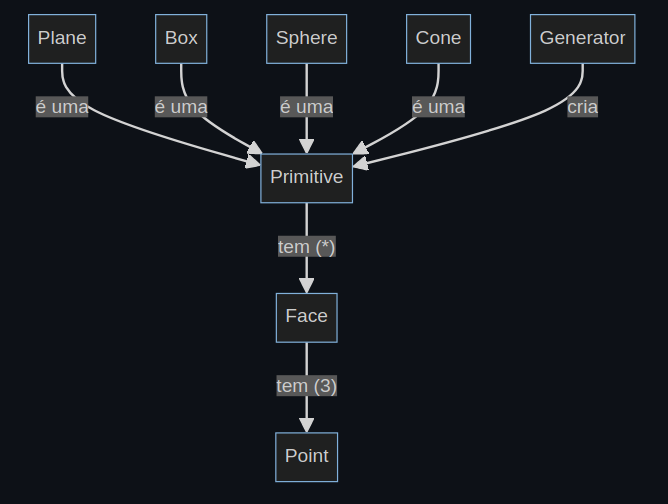
\includegraphics[width=\textwidth]{imgs/gendom.png}
    \captionof{figure}{Modelo de Domínio do Gerador de Primitivas}
    \label{fig:gendom}
\end{center}

\noindent
Criado este primeiro modelo, é possível perceber a hierarquia utilizada
para a sua definição.\newline
\break
\noindent
O gerador irá, portanto, ser responsável pela criação de primitivas que
serão definidas pelas respetivas faces, que por sua vez são constituídas
pelos seus pontos.\newline
\break
\noindent
Estas primitivas poderão ser do tipo \textbf{caixa, esfera, etc.} que,
por sua vez, definirão os processos necessários para a construção de pontos
e faces que bem definam a sua estrutura.

\subsection{Motor Gráfico}

\begin{center}
    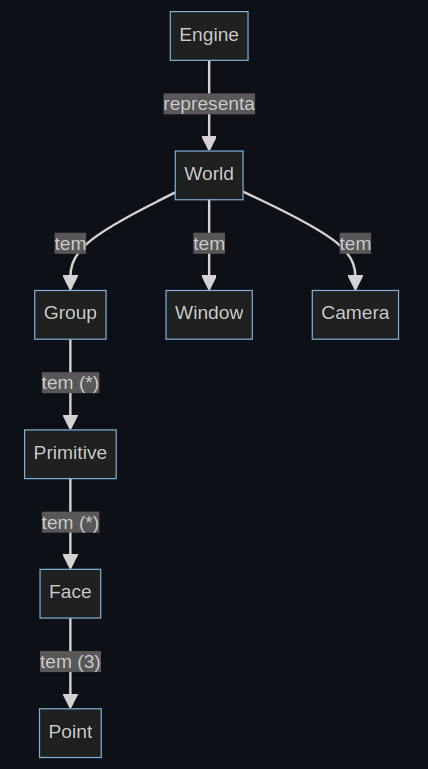
\includegraphics[width=0.7\textwidth]{imgs/engdom.png}
    \captionof{figure}{Modelo de Domínio do Motor Gráfico}
    \label{fig:engdom}
\end{center}

\noindent
Embora com um ramo semelhante, o motor intrepreta o seu domínio de maneira
diferente.\newline
\break
\noindent
O motor usará uma noção semelhante de primitiva, também, porém não utilizará
as definições mais especificas do que uma primitiva pode ser
(\textbf{esfera, etc.}), visto que as faces e pontos lidos dos ficheiros 
\textit{3d} deverão ser mais do que suficientes para a boa representação
das figuras pretendidas.\newline
\break
\noindent
Fará uso, ainda, de um mundo que possuirá um grupo de representação, uma câmera
e uma configuração de janela, em memória, que após lidos
da configuração \textit{XML} serão, posteriormente, utilizados
para a representação da configuração pretendida
pelo utilizador na janela e no cenário do motor.

